% Packages:

\usepackage{graphicx}

%%%%%%%%%%%%%%%
% Paper setup %
%%%%%%%%%%%%%%%

% What is your topic?
The topic of this paper is the environmental sustainability of vineyards within Australia.
% What is the context for your reserach?
The context of this research is that the Australian wine sector in general has gone through many tribulations due to economic, environmental and social pressures. Previously we attempted to highlight areas of concern through the use of statistical models, which were able to show strong correlations between various environmental and economic factors. However, discussions with industry and experts helped to identify that these relationships were not entirely causal, with some management and process of winegrowers obfuscating effects by directly addressing them. A key example of this was the lack of water use change during drought periods due to various methods that were used to obtain either more water or to circumvent the detrimental effects of lacking water resources.
% What do you want to achieve?
The identification of key factors; and their relation and contribution, direct or indirect, to the environmental sustainability of Australian winegrowing.
% Are there any relationships you want to explore?
This is key to this study. The relationships are in many ways more important to the research than the effects.

%%%%%%%%%%%%%%%%
% Working title
%
\title{Bayesian Networks for Assessing Environmental Sustainability in Australian Vineyards}

% Description
% NB Avoid titles along the lines of: “Effects of ...”, “The role of ...”, etc.  Be specific about the effect and its significance so that your reader knows what is on offer.

% For example, rather than write a title like “The effect of factor X on astrophysical properties of green cheese.”, 

% be specific about the effect and write something more like ...

% “Factor X halves the lunar thermal diffusivity of  green cheese”.

% You will usually find it easier to write an effective title if you make your title a sentence.

% Notes
% N/a

%%%%%%%%%%%%%%%%%%%%
% Intended readers
%
% David Klassen (wine maker Taylors)
% Dpt Agriculture - EL worker
        % They would like to know for policy
% Lawson - asked about OOBNs
% Winegrower - Someone from the limestones coast. The guy from Robe was interested.

% Description:
% Name 4 or 5 potential readers - give their names and why they would be interested  (e.g. “Ichabod Crane, paleo-fudgologist interested in polygalactic fudginomiality”, not “assorted paleo-fudgologists”).   

% Your readers should be outside your institution.

% Notes
% Many viticulturalists I know of are on the panel. It makes it hard to get one in particular.

%%%%%%%%%%%%%%%%%%%%%
% Anticipated Journal
%
% OIV Congress 2024

% TODO: The original conference has fallen through we will need somewhere else.

%%%%%%%%%%%%
% Question %
%%%%%%%%%%%%

% TODO: review the following questions:
What are the key factors/indicators of environmental sustainability in the australian winegrowing industry?
How can we measure and relate the factors that contribute to sustainability in the australian winegrowing industry?
What are the key factors that relate directly to environmental sustainability?
- and what in turn are the factors that contribute to these (and thus indirectly to environmental sustainability)?

% Things to consider
%
% Why is the knowledge important?
This was identified as a gap within our own prior research and is helpful in creating a basis for scenario assessment and comparison. This will allow a greater understanding of how these factors change within different scenarios; whether that be climate, region, business goal.
% What is the significance?
The significance is to bridge the gap between correlations and data to causal relationships. To inform growers using factors that are within their control, or how factors within their control are indfuenced by natural phenomenon.
% How will the findings be utilised?
These findings will be used to help inform the wider winegrowing community of what factors are most significant to environmental outcomes, and how they interact with one another. In practice this study aids a grower through informing them of how decisions impact environmental outcomes and how changing circumstance contribute to these factors and outcomes.
% What improvements may be derived from this result?
A wider more informed understanding of contributing factors to environmental impact and how different factors relate to one another to contribute to these findings.
% Are the terms well defined?
The terms are well defined. This was a key outcome of this project.
% Do experts think your question is important/relevant/doable?
Experts helped to guide this decision, and changed the trajectory of this project in response to data presented and how well they believed they could inform the study.

% What is the nature of your question?
%         who, what, where, when, why, how?
What are the key factors that contribute to environmental impact within the Australian winegrowing industry?
How do these key factors relate to each other and what are the factors that influence them?
What are the decision that can be made by growers that can change the environmental outcomes of their vineyards?
How do these factors chagne across well understood scenarios?
% You can have more than one question.

% What is the most important question your paper will pose?
What are the key factors to environmental impact within the Australian winegrowing industry, and how are these factors related?
% NB It is essential that your answer is framed as a direct question.  Your response must end with a question mark.

% Why is the question/issue/problem worth examining?
By examining the key and relevant factors to vineyards' environmental impacts we can better prepare for future changes in climate pressure, economic restrictions; that is we can better use this model to assess the potential environmental outcomes of the wine industry, as informed by experts, given potential upcoming challenges or changes.
% Briefly outline the problem you are tackling and explain why the problem is important to knowledge in general.  “Nothing much is known” is not sufficient justification by itself.  You have to show why the gap in knowledge is important.  Expect to draw heavily on your reading of the literature in framing your answer but do not get into detail of  author and year.
The collection of data and subsequent statistical analytics can only go so far as to fill the gap between cause and effects within wiengrowing. This research helps to fully understand the relevant decisions being made, how they are informed and what the known outcomes are. This helps to align these results to data collected to show stronger causal relationships than pure correlative, or hypothetical postulations of statistical analysis.
%%%%%%%%%%
% Answer %
%%%%%%%%%%

% What is the answer to question
%
% 
% NB  You must give a direct answer to the question posed.
% Notes

% Will the findings be considered significant?

% How did you gather the evidence? 
%
% Briefly outline the methods you used to gather your evidence.

% What is the main evidence?
%
% Briefly outline the key results.  Focus on outcomes.

% What can you add to theory?
%  
% A research paper has to add to broader understanding. What will yours contribute?  Think about how your results and conclusions will change how people see the world.
%
% Many people have trouble with this section.   Do not recycle the results.  Focus on the conceptual models that explain why your results are as they are, or why they are different from what might have been expected.  Your contribution may be something new or it may be confirmation of something already known but in a slightly different context.
%
% Sometimes the contribution to theory is not a simple answer but a better understanding of the questions that ought to be asked in future.
%
% Again, expect to draw heavily on the literature in framing your answer, but cite the literature only sparingly here (you can go into full detail when you prepare your discussion).

% What can you add to practice?
%
% Superior research also has practical consequences.  What are the consequences of your work?  Think about how your results and conclusions might change what people do. Do not merely restate your results.

%%%%%%%%%%%%%%%%%%%%%%%%%%%
% Significance and Impact %
%%%%%%%%%%%%%%%%%%%%%%%%%%%

% Highlight the importance of this

% Stress the practical implications and potential benefits for winegrowers.

%  Explain how your research could influence policy and practice?
% TODO: How is this done in academia? The result should be measurable? yet many papers do not have impact or it would be considered "industry"? what is the noemclature of this?

%%%%%%%%%%%%%%%
% Future work %
%%%%%%%%%%%%%%%

% What remains unresolved?
% 
% You may or may not have a lot to say here.  Some of it may be useful in your discussion.




%%%%%%%%%%%%%%%%%%%%%%%%%%%%%
%       Workshop ideas      %
%%%%%%%%%%%%%%%%%%%%%%%%%%%%%

% Ice breaker
% - who are you what are you involved in.
% Who knows who?
%

% Ask the expert team to nominate scenarios of interest then enter evidence into the BN to represent these scenarios.

%%%%%%%%%%%%%%%%%%%%%%%%%%%
% Notes for this article! %
%%%%%%%%%%%%%%%%%%%%%%%%%%%

% TODO: I believe this is the diary industry paper.

% The creation of the model was done in the following stages (this is on page xxiv):

%  + The conceptual model
%  + key sustainability indicators
%  + Connection of key indicators to available measurable variables

% The identified measurable variables were:

% Econoomy (Farm to gate was used):
%  + Economics
        % + Debt
        % + Assets
        % + Investment
%  + profitability
        % + Interest
        % + Income
        % + Competitiveness
% %  + Work force
%         + Employment
%         + Productivity
%         + Management
%  + market
        % + Commodity prices
        % + Supply
        % + Risks
%  + physicals
        % + Efficiency
        % + Resource
        % + Inputs
%  + commodity prices
%  + Supply and risks

% Social (across farm, factory and market)
%  + employment
        % + Labour
        % + Training
        % + Management
%  + legal and ethics
        % + Discrimination
        % + Compliance (regulatory)
%  + community
        % + Culture
        % + Value
        % + Cohesion (participation/social responsibility)
%  + health and safety
        % + Animal welfare
        % + occupational
        % + Consumer
%  + product
        % + Nutrition
        % + marketing

% Environment
%  + Reource Efficiency
%         + Water
%         + Energy & emissions
%         + land and soil
%  + Waste
%         + Water Waste
%         + Solid Waste

% A high | low | medium score was used

%%%%%%%%%%%%%%

% Introduction?

% This research provides valuable insights and data that can inform and guide decisions made by policymakers and industry leaders in the Australian winegrowing sector. By identifying key sustainability factors and their interactions, this study offers evidence-based recommendations that can support the development of more effective and sustainable agricultural practices and policies.

% The research for this project has identified that there is no uniform
% way to measure sustainability, no uniform agreement on indicators
% that could be used for measurement and even less agreement on
% which metrics should be used to quantify these indicators. This is
% best demonstrated that of the 72 triple bottom line frameworks, the
% indicator water occurred in 64 of these frameworks, although there
% appeared to be no standard metric identified to measure how water
% was measured. This is an endemic problem with sustainability
% measurement.

% The forces which drive the social, economic and environmental sectors, the decision-makers who have the power or influence to accept or reject change, cannot be ignored, if change is to be achieved (van Kerkhoff and Lebel, 2006).It may be that part of the problem with the progress of sustainable development in the past has been the traditional divide between those undertaking the systematic research and those on the ground required to take up and act on the results of such. The dissemination of research results has usually only occurred on completion, in a unidirectional, linear communication (van Kerkhoff and Lebel, 2006), whereas, as grounded researchers explain, the ownership of ideas and a willingness to implement these relies on a more collaborative approach from the outset, before research has even commenced. It requires acknowledging that experts exist in all spheres and need to be able to share information and debate, in order to come to agreement on issues, assessment tools, priorities for remediation and an optimal approach to solving problems (Corbin and Strauss, 2008; Johnson and Mengersen, 2009), e.g. improving sustainability.

% The sustainability Bayesian network model was constructed using
% open source software and has been delivered as a software package.
% A future project could focus on making it easier for a wider range of
% relevant stakeholders to engage with the model. For example a
% graphical user interface to the model could be developed and
% then web-enabled so that stakeholders can readily interact with the
% model and run scenarios.

% The concept of sustainability has been described as the most
% challenging policy concept ever developed (Spangenberg, 2004).
% There are more than 100 definitions of sustainability and sustainable
% development (Labuschagne et al., 2005). The most frequently cited
% definition comes from the pivotal 1987 World Commission on
% Environment and Development ‘Brundtland Report’, ‘development
% that meets the needs of the present without compromising the ability
% of future generations to meet their own needs’ (WCED, 1987).


% It is necessary to understand the impacts of each system on one another, for example, the impact of industries on climate change, diminishing resources, economic shifts and social change. In turn, it is necessary to understand the impact of variables such as these on an industry, its future viability, its surrounding communities and the economies they feed or depend on (Brundtland, 2007). Thus, a tool is required that can measure complexity within and between systems and model how changes in one element, positive or negative, might flow on to others. Only then can strategies for sustainability be developed with reduced risk of unintended negative consequences (Johnson and Mengersen, 2012).



%%%%%%%%%%%%%%%%%%%%%%%%%%%%

% references to check:


% https://www.sciencedirect.com/science/article/pii/S1462901122003872

%%%%
% A triple bottom line planning tool for measuring sustainability; A systems approach to sustinability using the Australian dairy industry as a case study.

% Capra, 1996; 
% Johnson and Mengersen, 2012)

% Murphy (2002)
%  A diagram of graphical models!

% The below references are from the previous OIV conference
%       Interestingly the theme was sustainability.

% 2023-3134: A DIGITAL TWIN APPLICATION FOR VINEYARDS SUSTAINABLE MANAGEMENT
% Vittorio Faluomi: Tecnovine srl, Italy, vittorio.faluomi@tecnovine.com

% 2023-3299: SUSTAINABLE PRODUCTION OF GRAPEVINE AND WINE IN TEXAS
% Amit Dhingra: Department of Horticultural Sciences, USA, amit.dhingra@ag.tamu.edu

% 2023-2958: DO SUSTAINABILITY CREDENTIALS NO LONGER SERVE AS A COMPETITIVE ADVANTAGE? - THE
% QUEST FOR COMPETITIVE PARITY WITH REGARD TO SUSTAINABILITY IN THE WINE INDUSTRY
% Barbara Richter: Hochschule Geisenheim University, Germany, barbara.richter@hs-gm.de

% 2023-3028: THE BLOCKCHAIN FOR THE SUSTAINABILITY OF DESIGNATIONS OF ORIGIN AND QUALITY AGRI-
% FOOD DISTRICTS: THE CASE OF VERMENTINO DI GALLURA D.O.C.G.
% Graziella Benedetto, Forleo Marina: University of Sassari, Italy, gbenedet@uniss.it

%  **************** This one looks super relavent
% 2023-3044: SUSTAINABILITY ASSESSMENT: TESTING AND VALIDATING A HIERARCHICAL FRAMEWORK IN THE
% PORTUGUESE WINE SECTOR CONTEXT.
% Ana Trigo, Ana Marta-Costa, Rui Fragoso: Centre for Transdisciplinary Development Studies (CETRAD), University of Trás-
% os-Montes e Alto Douro (UTAD)., Portugal, anatrigo@utad.pt

% 2023-3146: USER-GENERATED CONTENT AND RELEVANCE OF SUSTAINABILITY ATTRIBUTES FOR WINE
% CONSUMERS
% Miguel-Ángel Gómez-Borja, Inmaculada Carrasco, Juan-Sebastián Castillo: Universidad de Castilla-La Mancha, Spain,
% miguelangel.gborja@uclm.es

% 2023-2844: THE JOURNEY TO FARMLAND SOIL RESTORATION: UNDERSTANDING AND MEASURING
% PROGRESS TOWARDS SUSTAINABILITY
% Alberto Acedo: Biome Makers, Spain, acedo@biomemakers.com

% 2023-3239: ECOLOGICAL CRITERIA FOR A SUSTAINABILITY ASSESSMENT USING THE EXAMPLE OF THE ONLINE
% CERTIFICATION "NACHHALTIG AUSTRIA" (SUSTAINABLE AUSTRIA)
% Franz Rosner, Barbara Richter: Federal College and Research Institute for Viticulture and Pomology Klosterneuburg,
% Austria, franz.rosner@weinobst.at

% 2023-3084: THE IMPORTANCE OF RURAL EXTENSION AND ADVISORY SERVICES TO ACHIEVE A SUSTAINABLE
% VITICULTURE IN A CLIMATE CHANGE SCENARIO
% Ana Chambel: AVIPE, Portugal, ana.chambel@avipe.pt

% 2023-3220: EXPLORING BAYESIAN BELIEF NETWORK TO SUPPORT SUSTAINABLE VINEYARD IRRIGATION IN
% BRAZILIAN SEMI-ARID
% Luiz Gustavo Lovato: UNICAMP, Brazil, luizglovato@gmail.com

% PO-302
% 2023-2856: DATA DRIVEN APPROACH TO ENERGY EFFICIENCY IN WINERIES
% Gellio Ciotti, Marco Bietresato, Alessandro Zironi, Roberto Zironi, Rino Gubiani: Università degli Studi di Udine, Italy,
% gellio.ciotti@uniud.it



%%%%%%%%%%%%
% Definitions:

%%
% Iterative Bayesian network developement cycle
%
% \autocite{johnsonIntegratedBayesianNetwork2009}
% This article  illustrates a proposed integrated Bayesiannetwork  modeling  approach  using OOBNs within theiterative Bayesian network development cycle (IBNDC
% ^ This is a really comprehensive and well written definition of object orientated bayesian networks!
% 
%
%

%%
% integrated Bayesian networks
%
% The complex nature of environmental issues makes themideal case studies for the use of Bayesian networks as anintegration tool (Varis and Kuikka 1999; Uusitalo 2007;Barton et al. 2008), 
%
% Integrated models incorporate other types of tools like regression etc - it is literally what we are doing here. I would ask for a better definition from kerrie though. The term is used a lot but I cannot find an explicit definition.
%

%%
% Self-organising systems.
%
% Sustainability is one such complex system. It comprises complex interacting factors and processes (e.g. in the context of the dairy study: farm, factory and market processes; and environmental, social and economic factors). It is self-organising; it does not require external intervention to thrive or deteriorate (e.g. an ecosystem can be sustainable through self-organisation). It can also exhibit emergent behaviour, since intervening in one part of the sustainability system can have unintended and quite extreme effects in seemingly unrelated parts of the system (Johnson and Mengersen, 2012).
%
% These systems are exactly what you think they are. It is described in physics, chemistry, social sciences and philosophy.
% 
% The wiki is quite informative.
%https://en.wikipedia.org/wiki/Self-organization





% Initiatives to improve the environmental impacts of the Australian Wine industry have been ongoing since the 1990s; with recommendations to implement strategies for national programs that would help educate industry members in sustainable practices (Keith Jones, 2002). The first legislative initiative to support national programs was the Environmental Management Guidelines for Vineyards in Western Australia during 2002 (Nind, 2002). The first national program was the Australian Wine Industry Stewardship, beginning shortly after, during 2004 (WFA, 2009). This program was replaced multiple times during the 2000s, first by the Australian Wine Environmental Stewardship, and then by EnviroWine, finally becoming EntWine in 2009. The period in the 2000s was further influenced by several key researchers and program leaders, where concurrently multiple regions developed approaches to sustainable management tied to sustainability programs (SWA, 2023). EntWine was eventually acquired by the Australian Wine Research Institute and Australian Grape & Wine during 2015; which would lead to its redevelopment into Sustainable Winegrowing Australia (SWA) during 2019/2020 (SWA, 2023).
%             2.1.2. Previous Research and Motivation
% During the period of 2010 to 2023 data was collected voluntarily from wine industry members through the national sustainability programs, ultimately being in SWA possession as of 2023. The data set was used in 2020 to analyse sustainable practices, resulting in the development of a Resource Intensity Score (RIS); where the RIS was a summary indicator value of a vineyard’s energy use, emissions and water use (Nayak et al., 2020). The analysis then fit vineyards’ RIS values to 55 variables sourced from 23 separate wine regions during the period of 2015 to 2018 through the use of Stepwise Regression modelling. It was found that the top 10% gross margin vineyards had a lower operating cost and a lower RIS score than vineyards in the bottom 10% gross margin.
% The motivation for this thesis is to investigate the differences between the top 10% gross margin vineyards and those of the bottom 10%, hoping to uncover what the key differences were and to relate them to sustainable practices; as there is a known gap in the literature due to the difficulty to evaluate relationships using empirical evidence of both the environmental and economic impacts of sustainable practices in viticulture. This difficulty stems from data scarcity, industry complexity and transparency. While there have been attempts to fill these gaps, methodologies and indicators have lacked in ability to compare different regions and scales (Baiano, 2021).
%             2.1.3. Economic Pressures
% Historically strong demands for Australian wine have helped to create a thriving industry, however recently sharp reductions in exports to mainland China due to significant deposit tariffs have caused  a decline of 19% in Australian export value during the 2021-2022 financial year (see Figure 1) (Wine Australia, 2022). The pressure brought on by the drop in export value has been exacerbated by loss of tourism and labour due to the COVID-19 pandemic, global freight crisis, war in Europe and rising inflation (Wine Australia, 2021a, 2020). These pressures within the wine industry have trickled down to vineyards, where winemakers retain unwanted wine, creating an oversupply of grapes. Currently the proposed strategy to soften pressures proposed by Wine Australia includes initiatives focused on market diversification, and sustainability to build resilience in the coming years. 
% Figure 1:  The exports of Australian wine over time in Australian Dollars Free On Board, comparing exports between China and the rest of the world. This graphic is taken from the Wine Australia Annual Report of 2020-21(Wine Australia, 2022).
%             2.1.4. Environmental Pressures
% There are several environmental concerns that affect viticulture, including loss of soil quality, lack of rain, hail, disease, fire, and frost; with climate change exacerbating these issues. In 2020, 40,000 tonnes of grapes were lost across 18 different wine regions due to bush fires and smoke taint; the predicted incidence of wildfires is expected to increase (Canadell et al., 2021). In comparison to countrywide pressures such as drought, this damage made up only 3% of the total amount of grapes for that year; although acknowledged as a considerable loss on an individual basis, it was deemed to be only a minor national concern by Wine Australia when compared to other environmental pressures such as drought (Wine Australia, 2020). 



%
%This analysis addresses the knowledge gap regarding the effectiveness of regional level strategies employed in the wine industry and their relation to grape quality.
% What the hell is a regional strategy
% And how do you define, or know what trategy each region is using?
%
% Through the use of classification trees this study aims to highlight the key differences in sustainable practices at a regional level and how these practices relate to the different grades of grape quality.

% This does not really address what the methods are - aside from classisifcation trees in the most vague sense.
% What are the results briefly? why should someone read this article?
% What is interesting - what will be discussed in the article with regard to these results? What makes me want to read the article?
% And what is the take away point of the article? If I cant be bothered to read this article, what piece of knowledge can you leave mewiwth that I could recommend the article to someone else with?


\section{Methods}

In agriculture, the consideration of environment is critical to the success of the industry. The question of environmental sustainability has continued to grow in importance as the industry is affected by international market demands, disease pressures, natural disasters and social change \citep{wineaustraliaNationalVintageReport2022,wineaustraliaNationalVintageReport2020,wineaustraliaNationalVintageReport2021,cassonMultidisciplinaryApproachAssess2022}. The question of sustainability requires the consideration of a multitude of factors, not only due to physical differences between locations/habitats but also due to priorities driven by a myriad of perspectives from as consumers, ecosystems, government and industry \citep{baianoOverviewSustainabilityWine2021,wayeCarbonFootprintsFood2008}. It is important to consider each factor with respect to its relevant perspectives, and to be explicit in how each of these factors and perspectives are defined \citep{santiago-brownSustainabilityAssessmentWineGrape2015}.

Collaboration between experts from different perspectives is a useful method to reconcile opinions of the significance of different factors and their contribution to sustainable outcomes \citep{dichiaraCollaborativeApproachAchieving2024}. In Australia, the views of both industry and consumer are united in their priority to improve greenhouse gas emissions and resource inputs through approaches such as regulating chemicals, water use and fertilisers \citep{dumbrellComparingAustralianPublic2024}. While there is a general agreement on broader regulatory needs, the industry requirements vary greatly between different wine regions; due to climate, soil types and water resources \citep{abbalDecisionSupportSystem2016,agostaRegionalClimateVariability2012}.

Methods for measuring sustainability comprise a wide variety of approaches with the use of index systems being common \citep{gehringerMappingSustainabilityMeasurement2024}. Other approaches utilise the identification of key factors, and their measurements as a proxy to indicate impact to, or the health of, the environment \citep{floresWhatSustainabilityWine2018}. The measuring of sustainability through the use of these tools can help to manage risk and promote resilience for industries through identifying sustainable goals and key factors of interest that contribute to positive outcomes \citep{klemesAssessingMeasuringEnvironmental2015, beckerSustainabilityScienceManaging2024}. Within this study we focus on measuring key factors and establishing how they interact, and ultimately effect the surrounding environment; the chosen method for this study is a Bayesian Network.

\subsection{Literature Review}
#TODO:

\subsection{Bayesian Networks}

A Bayesian Network is a graphical model, being comprised of nodes and edges. Uniquely, Bayesian Networks contain the network's operations within the nodes themselves instead of across the edges. This is done in the form of probability tables, with connections being informed by the edges. There is simplicity within the calculations done within a node, as it is fundamentally achieved through sum and division operations. However, great complexity is introduced when a node is informed by many parents, which can also have many parents themselves. The change in a single parent node effects all children of the network; often resulting in intractable systems, especially when nodes may have numerous classes \citep{korbBayesianArtificialIntelligence2011}. The strength of this complexity over simple operations, is the ability to encapsulate incredibly complex systems with simple definitions.

The use of a Bayesian Network allows for the ability to include perspectives from industry experts and create a causal structure. The graphical nature of the Bayesian Network also helps to illustrate factors within the model and communicate the complexity and relationships of factors to one another; and ultimately a factor's relation direct or indirect, to a vineyard's environmental impact \citep{pourretBayesianNetworksPractical2008}. Furthermore, data collected across Australia could also be used to help inform both scenarios and the model alongside expert opinion.

The calculations of a Bayesian Network are based on Bayes' theorem, shown as follows
\begin{equation}\label{bayesformula}
P(A|B)= {P(B|A)P(A)}\over{P(B)}
\end{equation}.
Where we calculate the probability of an event A given an event B, as demonstrated by \cite{bayesLIIEssaySolving1763}. Within a Bayesian Network, an event can be considered any given node and its outcome one of the node's classes. Events are connected by edges within the network, with each node containing the probability of an outcome given parent nodes' outcomes. This is an iterative application of \ref{bayesformula}, which can be achieved through

\begin{equation}
        \mathbb(P) (X_{1}=x_{1},...X_{n}=x_{n})=\prod_{n}^{i=1}p(x_{i}|x_{Parents(i)})
\end{equation},
for a selected node $i$ given the parents and their local conditional distributions.

The iterative nature, or the ability to show the difference in probable outcomes of different sets of events and their uncertainty allows for the ability to conduct inference. This type of Bayesian inference shows the difference between the likelihood of various outcomes with and without different evidence of prior nodes outcomes being present. The sets of different outcomes then stored as a joint probability distribution, which can be decomposed into the conditional probabilities of each set of possible events occurring and their likelihoods.

One of the greatest abilities within this style of inference is Marginalization. In which, the outcome of a particular event can be determined irrespective of other outcomes. This type of marginalisation is intuitively represented as nodes conditional independence is illustrated inherently through the structure of the graph by its edges.

Bayesian Networks created in this study were created using BayesFusion \citep{bayesfusionGeNIeModelerUSER2022} to calculate the networks and their probabilities. The use of Bayes fuse software was used both through the GUI interface and the SMILE API \citep{bayesfusionGeNIeModelerUSER2022} system using C++ \citep{ISO:2012:III}.

\subsection{Elicitation}

The Bayesian Network was constructed using a mixture of data and expert elicitation. The format followed recommendations from \cite{korbBayesianArtificialIntelligence2011,pitchforthProposedValidationFramework2013}. Where, we progressed iteratively through from problem definition, to structure, to parametarisation, and then to validation. Experts were initially informed regarding the process to establish an understanding of what each step would be comprised of, as well as highlighting common pitfalls and how we would address them. With common problems being listed by both authors being:
\begin{enumerate}
        \item Not understanding the problem context
        \item complexity without value
        \item Getting arc directions wrong
        \item too many parent nodes
        \item Bias expert estimates
        \item Inconsistent probabilities
        \item Being absolutely certain
\end{enumerate}
To address these issues, experts were kept well-informed of them, as well as variable definitions and problem scope. Open communication was maintained during the entire process to help answer questions regarding the model, process, and to maintain transparency. Communication included in-person and electronic one-on-ones and group sessions; with elicitation of expert knowledge being primarily conducted through a series of workshops with the panel of industry experts.

Each workshop had a primary focus such as: scope, structure or parameterisation; with, prior concepts being built upon iteratively. The first important establishment was the scope of the network, and how well it could or couldn't be adapted to a wide variety of circumstances within the Australian winegrowing industry. Following this was the discussion around the structure of the network, which entailed the description of relationships and stricter definitions of each factor to one another. Finally, variables were paramatised using conditional probabilities.

To introduce new concepts and how they interacted, preliminary simplified versions (strawman examples) were provided to experts; with the intention of these examples to be examined, critiqued, and improved upon. The use of these strawman examples enabled a more engaged and effective review process. Experts were initially able to interact with elements of the model and see how they worked together. The strawman examples were crafted from a foundation of literature and data to offer a basic, layman's understanding of key factors and concepts, serving as a starting point for further development and discussion. 

\subsection{CPT interpolating}

As is often the case, the most arduous endeavour is to attribute probabilities to events defined within the Bayesian Network \citep{korbBayesianArtificialIntelligence2011}. Due to the growing complexity of the network throughout the study each event was described by binary classes. With the classes depicting a positive or negative contribution to a vineyard's environmental outcome. Furthermore, the complexity of the variables, particularly water use, were overwhelmingly interrelated to operations across the vineyard. To attempt to capture this complexity but not dilute the ability to work with various scenarios the conditional probabilities were interpolated.

This method utilised interpolation between two anchored points. One point represented the case of all factors being true/positive and the other represented all factors being false/negative. The interpolation was achieved by designating each factor an attributed weight; where, weights were indicative of a factor's overall influence to its child node. During workshop discussion participants were the most comfortable using scores out of 10 to describe a factor's influence on its child node.

Using this method, any given probability can be calculated using
\begin{equation}
        p=x\sum_{i}^{n} + y\sum_{m}^{i} 
\end{equation},
for n number of true or contributing factors and m false or not contributing factors. We know the solutions for when all contributing factors are true ($p_t$) or all were false ($p_f$). Where,
\begin{equation}
        p_t=x\sum_{i}^{n} 
        \text{ and }
        p_f=y\sum_{m}^{i}
\end{equation}.
From here values for $x$ and $y$ are able to be derived using the sum of the provided weights.

\subsection{Validation}

The method for validation sought to address concerns presented by \citep{pitchforthProposedValidationFramework2013}; who listed the following:  nomological, face, content, concurrent, convergent, discriminant and predictive validity. Validation steps were partly incorporated during the process of constructing the Bayesian network itself. Specifically when considering the nomological validity of the network; the expert panel was asked directly regarding its ability to extrapolate beyond a single region, or scenario. In part, the selection process for experts, aspired to be diverse within their regional knowledge and expertise in an attempt to broaden the ability to critique choices. Although it was agreed that multiple scenarios were well captured by the trees structure, minor additions would be needed to encapsulate the differences between specific winegrowing regions. This requirement aligned with literature, which highlighted how regional variation is considered a driving factor for many vineyard outcomes and priorities \citep{abbalDecisionSupportSystem2016,agostaRegionalClimateVariability2012,soarClimateDriversRed2008}.

The Face and content validity of the network was questioned directly by the expert panel through the structure and conditional probability phases. The choice of binary discretisation was due to two reasons; that it captured the relevant contribution to the node in question and limited the model from becoming to overly complex and circumstantial. This helped to avoid some overtly specific scenarios in favour for broader vineyard decisions, whilst allowing the model to address these behaviours in the future by specifically targeting a region and incorporating its considerations. This approach went hand in hand with the content validation. Where, it was found that the limitation of the model was primarily regional, which aligned again with the findings of other researchers \citep{abbalDecisionSupportSystem2016,ellisUsingBayesianGrowth2020,agostaRegionalClimateVariability2012,barriguinhaVineyardYieldEstimation2021,brockRelationSoilOrganic2011}. Specifically, the question of water resources, which was central to the model and highly interrelated \citep{carmonaUseParticipatoryObjectOriented2011}.

Similarly, the convergent validity of the model was accomplished through the broader discretisation of nodes into the binary forms of positive and negative affects on the environmental impact of the vineyard. This manner of discretisation allowed a clear delineation in localised subnetworks within the model. The alignment of the model to other research helped to further answer questions of concurrent validation. In that, it was found that other studies emphasised the same variables selected by our experts. This was especially true regarding the consideration of yield and regional factors that influence vineyard outcomes \cite{abbalDecisionSupportSystem2016,campsGrapeHarvestYield2012,hallWithinseasonTemporalVariation2011}. Furthermore, these types of variables are highly prevalent in greater agriculture studies that emphasise general outcomes and resource use such as yield and water respectively \citep{heFruitYieldPrediction2022,laurentLocalInfluenceClimate2022}.

The discriminant validation of the model was the most difficult, as the definitions of each node changed over the course of the model's inception. This brought the difficulty that nodes connected by edges would have to be reconsidered each time a definition changed. This issue was simply overcome through explicit definitions accessible to all participants, and by directly addressing issues caused by definitions before further development of the model. Again, the simplicity of binary state nodes helped to isolate definitions more distinctly, as well as employing methods such as node splitting, removal and adding additional nodes \citep{korbBayesianArtificialIntelligence2011}.

The structure of the model itself was similar to other models in the presence of variables but differed in some of their relation due to the terminal node being environmental impact. The paramitisation of the nodes did differ to other studies, as every node was related and thought of with regard, to the terminal node and how they subsequently affected the environmental outcomes of a vineyard and not other more prevalent outcomes such as yield \citep{laurentReviewIssuesMethods2021}. The discriminant validity of the model was highlighted through the acknowledgement of the model's requirement to be tuned to any specific wine region before being able to be properly employed. Furthermore, the predictive validity was able to be well established through two methods, the use of a case study and the consideration of extreme outcomes.

\subsection{Sensitivity analysis}

The sensitivity analysis conducted in this study utilised the Bayesian Network software GeNie, implementing the algorithm developed by \cite{article}; an optimisation of \autocite{Castillo1996ANM} and \cite{Gaag1998PracticableSA}. The method allows for efficient computation of the influence of parameter variations on the output probabilities of a Bayesian network, making it particularly suitable for complex models. Sensitivity was calculated on the terminal node 'Environmental Impact' to reflect its sensitivity to changes in other nodes.

The process utilises two outward and an inward propagation across a junction tree, a data structure representing the Bayesian network. These propagations are essential for establishing the necessary cliques that allow for the calculation of the sensitivity function using the coefficients $\gamma$ and $\delta$.

These coefficients are used in determining evidence through

$$ y = {{p(a, e)(x)}\over{p(e)(x)}}={{\alpha x + \beta}\over{\gamma x + \delta}} $$.

Where $y$ is the posterior marginal of interest, given evidence $e$, with respect to the parameter $x$. 

% FIXME: should I extrapolate on this method?

% y - a posterior marginal of interest
% e - evidence
% x - all possible probability parameters
% a - node of interest
% $$ y = p(a|e)$$

% $$ y = \alpha x + \beta $$

% marginal distribution of any given parent node of a - any given node parent of a
% b - the ith given parent node of a
% pi - the parent nodes of the b ith node
% $$ x = p(b_{i}|\pi) $$



% $$ p(e)(x) = \gamma x + \delta $$

% For each parameter under investigation, the sensitivity function 
% $$ y=\alpha x + \beta x $$

% y=αx+βγx+δy=γx+δαx+β​ is determined, where yy represents the posterior marginal probability, and xx is the parameter in question. The coefficients (αα, ββ, γγ, δδ) in this function are computed using the results from the propagations, ensuring computational efficiency.

The methodology is extendable to n-way sensitivity analysis, allowing for the examination of the joint effects of multiple parameters. This involves identifying the relevant parameters and their influence on the posterior marginals using the same propagation strategy multiple times.

By employing this method, the sensitivity analysis avoids the extensive computational demands of traditional brute-force approaches, which require numerous network evaluations. Instead, this approach ensures that all potential parameters are considered with minimal computational overhead; allowing the use of multiple scenarios based off different evidence.

\subsection{Case study: Coonawarra}

Due to the regional limitations of the model experts proposed a case study of a specific and well understood region: Coonawarra in South Australia. The choice of the region was due to the prevalence of data within and around the region, as well as experts' understanding of the region's unique challenges and benefits to winegrowing. The Coonawarra model was built off of the original Bayesian Network's structure with site specific conditional probabilities being entered and scrutinised by the expert panel.

% \citep{mayfieldDesigningExpertledBayesian2023} -> this reference also uses a similar method which we can cite alongside everything else.
% % These are transcribed notes from Korb & Nicholson:

% \citep{korbBayesianArtificialIntelligence2011} Korb & Nicholson describe three major issues in the creation of Bayesian Networks though knowledge Engineering:
% - Generating Arc Structure
% - Parametarisation
% - dealing with utilities

% Each element within the elicitation process was iteratively 
% Elicitation was conduct ach  Although workshops focussed on a single issue, it was important to continually address each issue in an iterative fashion. The approach to ensuring a sound and sane network, was to directly address common issues that occur during the construction of Bayesian Networks using ellicitation as outlined by #TODO: Korb and Nicholson. These issues are similarly highlighted by #:TODO: Pitchforth.

Transparency with the expert panel was a key ingredient with this approach, highlighting explicitly what these problems were and how we would overcome them. This included agreeing upon definitions of each node before connecting edges between them.

Although originally multiclass nodes existed, the bayesian network was altered to only include binary class nodes. Each edge between a node had to answer the following questions:
\begin{enumerate}
        \item Are the nodes in the BN the right ones?
        % \item Are the state spaces (values) for each node correct?
        \item Are the arcs right?
\end{enumerate}
If the answer to any of the above questions was no; then the structure was not considered sufficiently defined. Although we explicitly defined the structure of the BN prior to CPT parametarisation. This process continued when adding conditionaly probability values. The entire process of construction iinvolved the steps:
\begin{enumerate}
        \item exposing the panel to a strawman argument/model/definition
        \item Outlining the model and the process involved in defining the structure of a BN
        \item The expert panel reviewing possible nodes and arcs and definitions
        \item Defining their own structure, node or term.
        \item Agreeing upon the final definition, structure or model.
\end{enumerate}
\subsubsection{Trying to build the full model all at once}

Korb & Nicholson say that it is nearly impossible to build a complex BN all in one go. They recommend:
\begin{enumerate}
        \item dividing models into subcomponents
        \item breaking down the problem into a single target variable
        \item reducing the scope of the problem
        \item Setting a single time frame for the problem
\end{enumerate}
The strawman was presented as three subcomponents that pertained to the triple bottom line's environment, economy and social aspects.
Within the first workshop it was agreed on by the expert panel to reduce the scope from a triple bottom line to only reviewing the environmental impacts of vineyards. This also reduced the BN to a single terminal node. It was further decided to create the BN as a single season to limit its complexity.

\subsection{The problem}
\subsubsection{Not understanding the problem context, complexity without value.}
It is crucial to gain a clear understanding of the problem and its context. This can be seen as answering the following questions:
\begin{enumerate}
        \item what do you want to reason about?
        \item What dont you know?
        \item What information do you have?
        \item What do you know?
These questions are well addressed in prior research. The creation of baseline models showed strong linear relationships between many variables. The creation of XGBoosted trees uncovered the ability to well inform any particular variable but with no real causal structure or understandability. here we seek to pursue causality and link these variables together in a way that is more aligned with a decision support structure than purely as a predictive exercise.
\subsubsection{Complexity without value}
A very common impulse, when something is known about the problem, is to want to put it in the model. But including everything known, just because it is known, simply adds complexity to the model without adding any value (and in fact often reduces value). Instead, the knowledge engineer must focus on the problem:
"Which of the known variables are most relevant to the problem?"
- This issue in its the simplest form has attempted to be overcome through trying to mediate the workshop and inform experts of the potential probelsm that will come with a cumbersome model.
\end{enumerate}

\subsection{Structure - Nodes}
The list below is each of the problems, which can be addressed together in some fashion as the approaches of solving them overlap.
\begin{enumerate}
        \item Getting the node values wrong
        \item Node values aren't exhaustive
        \item Node values aren't mutually exclusive
        \item Incorrect modelling of mutually exclusive outcomes
        \item Trying to model fuzzy categories
        \item Confusing state and Probability
        \item Confusion about what the node represents
\end{enumerate}
Two major strategies were employed to overcome these problems. Tying nodes explicitly to a data source that corroborated the definition and state in some manner as the node. For node s that did not have data set they were sought to be defined with an explicit explanation that experts agreed upon or had some external explanation such as legislation.

\subsection{Structure Arcs}
\subsubsection{Getting the arc directions wrong}
Arc directions are commonly wrong for the following reasons:
\begin{enumerate}
        \item Modelling reasoning rather than causation
        \item Inverting cause and effect
        \item Missing variables
\end{enumerate}
To note: Korb and Nicholson do not actually suggest a method for overcoming these problems. There is an inherint risk in creating a model and not having knowledge of a missing variable or of a causation. It is important to acknowledge that there is always a possibility that causation is mixed up with reasoning, and that not all variables are always known.
\subsubsection{Too many parents}
Sometimes it is unavoidable that a node is affected by many factors, or other nodes. There are some methods to help overcome this such as divorcing, in which a node is created to capture the cumulative affects of several parents on a child. This technique was employed in the creation of the structure of the BN with the expert panel.

\subsection{Parameters}
\subsubsection{Experts estimates of probabilities are biased}
\begin{enumerate}
        \item Overconfidence: The attribution of higher than justifiable probabilities to nodes/events.
        \indent The tendency to attribute higher than justifiable probabilities (\citep{lichtensteinCalibrationProbabilitiesState1982} 
        \item Anchoring: The tendency towards higher/lower based off of an arbitrary point of comparison. "Anchoring" people at a higher or lower than normal prediction because of some assumption or example  \citep{kahnemanPsychologyPrediction1973}.
        \item Availability: The assessing of an event as more probable than is justifiable becaues it is more memorable or noticeable \citep{tverskyJudgmentUncertaintyHeuristics1974}.

\end{enumerate}
We have attempted to overcome this with two methods. A diverse and varried expert panel. Those participanting have experience in multiple vineyards as managers and other duties as well as the panel itself having varied manager/owners from different regions and scale. With some experts being more specialised in specific areas such as agro-chemicals.
\subsubsection{Inconsistent probabilities}
The collection of probabilities for when the CPT is large can result in inconsistent probabilities. The collection of probabilities at different times or if probabilities are supplied by different experts can result in inconsistent probabilities as well.
The use of desciptors such as very high or low can be of assistance \cite{vandergaag2013elicit}. In this study we overcame this through the use of worded response such as high and low. We then assigned probabilities to those broader cases. We had every expert agree upon each of the probabilities so that they could argue for or against any particular bias and so that the probabilities would even out to a more broader applicability, across all of the experts experiences.
% \item Inconsistent "filling in" of large CPTs:
-       -       - Being dead certain.
\subsubsection{Incoherent probabilities (not summing to 1)}
We used software that automatically detected incoherent probabilities when filling in the CPT values to overocme this problem.
\subsubsection{Being dead certain}
It is important that we limit over confidence (A quote form mark twain was used in the korb and Nicholson). 
Our best defence against this was to use multiple experts with different experiences and to challenge them when something was certain. To ask why and to check in about their thoughts.

\citep{morganUncertaintyGuideDealing1990}
Two attributes of good elicitation process are:
\begin{enumerate}
        \item The expert should be apprised of what is known about the process, especially the nearly universal tendency to overcomefidence and other forms of bias. In order to avoid some problems, values should be elicited in random order and the expert not given feedback on how the different values fit together until a complet set has been elicited.
        \item The elicitation process is not simply one of requesting and recording numbers but also one of the refining the definitions of variables and terms to be used in the model. What values are elicited depends directly upon the interpretation of terms and these should be made as explicit as possible and recorded during the elicitation. This is part of the process management described earlier.
\end{enumerate}
- 

\citep{Boneh2021} Boneh, T. (2010). Ontology and Bayesian decision networks for supporting the meterological forecasting process. Ph. D thesis, Clayton School of infomration technology, Monash university
Boneh 2010 describe Knowledge Engineering with Bayesian Networks (KEBN) as occurring in a 4 stage life cycle:
- Bayesian Network Structure
- Probability Parameters
- Decision Structure
- Utilities Preference

Pitchforth \citep{pitchforthProposedValidationFramework2013} agrees with this style of structure naming these steps as:
- Structure
- Discretisation
- Parametarisation
- Model behaviour
- Validation

Korb & Nicholson have a similar view to Pitchforth. utilising a waterfall style developemental approach which include 5 stages:
- Building the BN
-       - Structure
-       - Parameters
-       - Preferences
- Validation
-       - Sensitivity Analysis
-       - Accuracy testing
- Field testing
-       - Alpha/Beta testing
-       - Acceptance testing
- Industrial use
-       - Collection of Statistics
- Refinement
-       - Updating procedures
-       - Regression testing

Where discretisation and validation are additional steps to assign intervals to continuous factors (discretisation) and to ensure the models appropriateness (validation)

With validation incorporating the expert scrutiny of the models begaviour for scenarios, as well as comparing this to both data and other literature.

\subsection{Structure and Conditional Probabilities}

\subsection{Validation}

\citep{korbBayesianArtificialIntelligence2011}




% Abstract

1. Introduction to Methodology

    Brief overview of the research approach and the rationale behind using a Bayesian Network (BN) model for sustainability assessment in viticulture.
    Mention of the collaborative expert elicitation process and the sequential workshops that shaped the model development.

2. Identification of Sustainability Indicators

    Description of the process for selecting sustainability indicators, including the use of data from Sustainable Wine Australia.
    Criteria for indicator selection, focusing on relevance to environmental, economic, and social dimensions of sustainability in winegrowing.

3. Expert Elicitation Process

    Overview of the expert panel composition and the expertise represented.
    Objectives and structure of the expert elicitation process, highlighting the series of workshops conducted.

Workshop 1: Variable Review and Straw Man Model Introduction

    Objectives: To agree on the sustainability indicators and introduce the initial straw man model.
    Activities: Discussion on indicator relevance and definitions; presentation of the straw man model.
    Outcomes: Agreement on initial set of variables and conceptual understanding of the model's direction.

Workshop 2: Model Structure Refinement and Interpolation Method Introduction

    Objectives: To refine the model's structure and address the complexity of CPTs through an interpolation method.
    Activities: Examination of variable relationships; identification of complex CPTs; proposal of the linear interpolation method.
    Outcomes: Revised model structure; decision to develop and implement the interpolation method for complex CPTs.

Workshop 3: Finalization of CPTs and Case Study Selection

    Objectives: To finalize CPT values using the interpolation method and select a case study for model application.
    Activities: Presentation and application of the interpolation method; finalization of CPT values; selection of the Coonawarra wine region for the case study.
    Outcomes: Completion of model parameterization; selection of case study region emphasizing the model's practical application.

4. Development and Implementation of the Interpolation Method

    Detailed explanation of the linear interpolation method developed to manage the complexity of CPTs for variables with extensive connections.
    Justification for choosing this method and its anticipated impact on the model's usability and accuracy.

5. Case Study Application: Coonawarra Wine Region

    Rationale for selecting the Coonawarra wine region as a case study to apply and test the BN model.
    Brief description of how the model was applied to this specific context, including any regional data used and adjustments made for the case study.

6. Model Validation

    Overview of the validation process employed to ensure the accuracy and reliability of the BN model.
    Description of internal and external validation measures, including expert review and comparison with independent datasets.

7. Conclusion

    Summary of the methodological approach, emphasizing the collaborative expert elicitation process and the innovative solutions developed for model construction and parameterization.
    Brief mention of the significance of the methodology for sustainability assessment in viticulture and potential implications for future research and practice.

\section{Results}

\subsection{Industry definitions}

How can these key factors be rigorously defined so that they are quantifiable contributions to environmental sustainability?
Purpose: Develop the factors into well-defined and measurable impacts on environmental sustainability.
Results: Use the agreed upon definitions to fully realise factors and their impact.

% Please add the following required packages to your document preamble:
% \usepackage{booktabs} TODO: check the BN definitions align properly.
\begin{table}[h]\label{tab:definitions} 
    \begin{tabular}{@{}llll@{}}
    \toprule
    \textbf{Variable name} & Definition & \textbf{Ideal Class} & Not Ideal Class \\ \midrule
    \textbf{Water use} & Total amount of water used by a vineyard in a financial year (ML/Ha) & \textbf{Low} & High \\
    \textbf{Agrochemical type} & When selecting agrochemicals, those which are less hazardous to beneficial organisms and/or have a lower environmental impact are considered & \textbf{Yes} & No \\
    \textbf{Spray application number} & Number of foliar spray applications used to control pests and diseases (spray applications/Ha/FY) & \textbf{Low} & High \\
    \textbf{Agrochemical legislation} & The legislated regulations regarding agrochemical use as specified by the APVMA. Dog book recommendations are further restrictions for export wine production and to protect the reputation of Australian wine. & \textbf{Yes} & No \\
    \textbf{Vineyard floor management} & Proportion of vineyard floor covered with a cover crop. & High & \textbf{Low} \\
    \textbf{Pest and disease management methods} & All available methods of management are considered before a management program is chosen (i.e. biological, chemical, cultural, mechanical, and technological) & \textbf{Yes} & No \\
    \textbf{Electricity use} & Total amount of electricity used by a vineyard in a financial year (kWh/Ha) & \textbf{Low} & High \\
    \textbf{Electricity Price} & The unit cost of electricity purchased by a vineyard & \textbf{Low} & High \\
    \textbf{Renewable energy} & Percentage of energy that is renewable & High & \textbf{Low} \\
    \textbf{GHG emissions} & Total amount of GHG emission produced by a vineyard in a financial year (Kg CO2e/Ha) as calculated  by NGA legislation & \textbf{Low} & High \\
    \textbf{Environmental Impact} & The positive/negative impact a vineyard has on its immediate environment (to gate). & \textbf{Ideal} & Not Ideal \\
    \textbf{Fertiliser use} & Total amount of nitrogen (synthetic and organic) used by a vineyard in a financial year (Kg/Ha) & \textbf{Low} & High \\
    \textbf{Fuel use} & Total amount of fuel (diesel, petrol, lpg and biodiesel) used by a vineyard in a financial year (L/Ha) & \textbf{Low} & High \\
    \textbf{Renewable Fuel} & Percentage of fuel used that is renewable. & High & \textbf{Low} \\
    \textbf{Grape Price} & Grape price per tonne & High & \textbf{Low} \\
    \textbf{Nutrient leaching management} & The depletion of nutrients in the grapevine root zone is minimised through best practice irrigation scheduling and soil moisture monitoring. & \textbf{Yes} & No \\
    \textbf{Market supply and demand} & The relationship between the quantity of winegrapes produced and the quantity that consumers wish to buy & High & \textbf{Low} \\
    \textbf{Pest and Disease Management} & The management of pests and diseases such as through the employ of fungicide and pesticides & \textbf{Yes} & No \\
    \textbf{Soil degradation management} & Areas at risk of degradation via compaction or erosion are identified and actions to remediate and minimise degradation are taken (i.e. don’t traffic waterlogged soils, minimise cultivation, maintain vineyard floor cover with cover crops, etc.) & No & \textbf{Yes} \\
    \textbf{Soil organic carbon management} & Areas with low or declining soil organic carbon levels are identified and actions to improve soil carbon levels are taken (i.e. minimise cultivation, maintain vineyard floor cover with cover crops, apply mulch or compost, etc.) & \textbf{Yes} & No \\
    \textbf{Tractor passes} & The number of times a tractor passes over the whole vine row area & \textbf{Low} & High \\
    \textbf{Water use efficiency} & The amount of water used per tonne of grapes produced & High & \textbf{Low} \\
    \textbf{Water licences} & Current water licences and permits are adhered to & \textbf{Yes} & No \\
    \textbf{Water Price} & The cost per unit of water paid for by a vineyard & \textbf{Low} & High \\
    \textbf{Water quality} & Water used for irrigation is assessed annually for quality (pH, chloride, sodium absorption ratio, electrical conductivity, soluble solids, hardness, microbial contamination). Water that may case soil degradation or irrigation inefficiency is treated before use. & \textbf{Yes} & No \\
    \textbf{Water Scarcity} & Whether the country is suffering drought or not (s defined by BOM) & No & \textbf{Yes} \\
    \textbf{Weather Conditions} & A vineyard’s regional climatic conditions. & \textbf{Ideal} & Not Ideal \\
    \textbf{Grape quality and yield targets} & The yield and quality targets of a vineyard block as outlines in the grape supply contract. & \textbf{Ideal} & Not Ideal \\
    \textbf{Agrochemical score} & Agrochemicals with high human and environmental hazard scores are avoided. & \textbf{Yes} & No \\ \bottomrule
    \end{tabular}
\end{table}

The key factors identified were defined as shown in Table \ref{tab:definitions}. By utilising these definitions, each factor's contribution to environmental sustainability was assessed. The definitions provided a clear framework for measurement, ensuring that the factors could be consistently evaluated.

The quantification of each factor allowed for a systematic analysis of their impacts. For example, "Water Use" was quantified as "High" or "Low," enabling a straightforward assessment of its environmental impact. Similarly, other factors were defined and quantified to ensure their contributions to sustainability were measurable; with each being of the two general categories ideal and not ideal (low and high respectively for water use).

By applying these definitions, the study effectively translated the qualitative aspects of environmental sustainability into usable metrics. This approach not only facilitated a comprehensive analysis of the factors but also identified their specific relationships.

The use of these definitions enabled each of the factors' impacts to be linked and reviewed, demonstrating their importance in achieving environmental sustainability; allowing each factor's contribution to be clearly understood and relationships  explicitly defined.

\subsection{Comparative Analysis of Literature and Industry Perspectives}
    What are the factors of environmental sustainability in the Australian winegrowing industry?
        Purpose: Explore and understand the both the literature and industry perspectives on this.
        Results Literature review. Industry list of factors. Mind Map? Leximancer network.
        - Use the same words as the definitions in the search to show the parralels and differences.

% Please add the following required packages to your document preamble:
% \usepackage{booktabs}
\begin{table}[h]\label{tab:lexi}
\begin{tabular}{@{}lrr@{}}
\toprule
\textbf{Concept} & \multicolumn{1}{l}{\textbf{Count}} & \multicolumn{1}{l}{\textbf{Relevance_percentage}} \\ \midrule
water & 1321 & 100 \\
change & 817 & 62 \\
climate & 789 & 60 \\
disease & 646 & 49 \\
change & 569 & 43 \\
grapevine & 565 & 43 \\
viticulture & 565 & 43 \\
soil & 450 & 34 \\
plant & 425 & 32 \\
different & 300 & 23 \\ \bottomrule
\end{tabular}
\end{table}

\begin{figure}[h]
    \centering
    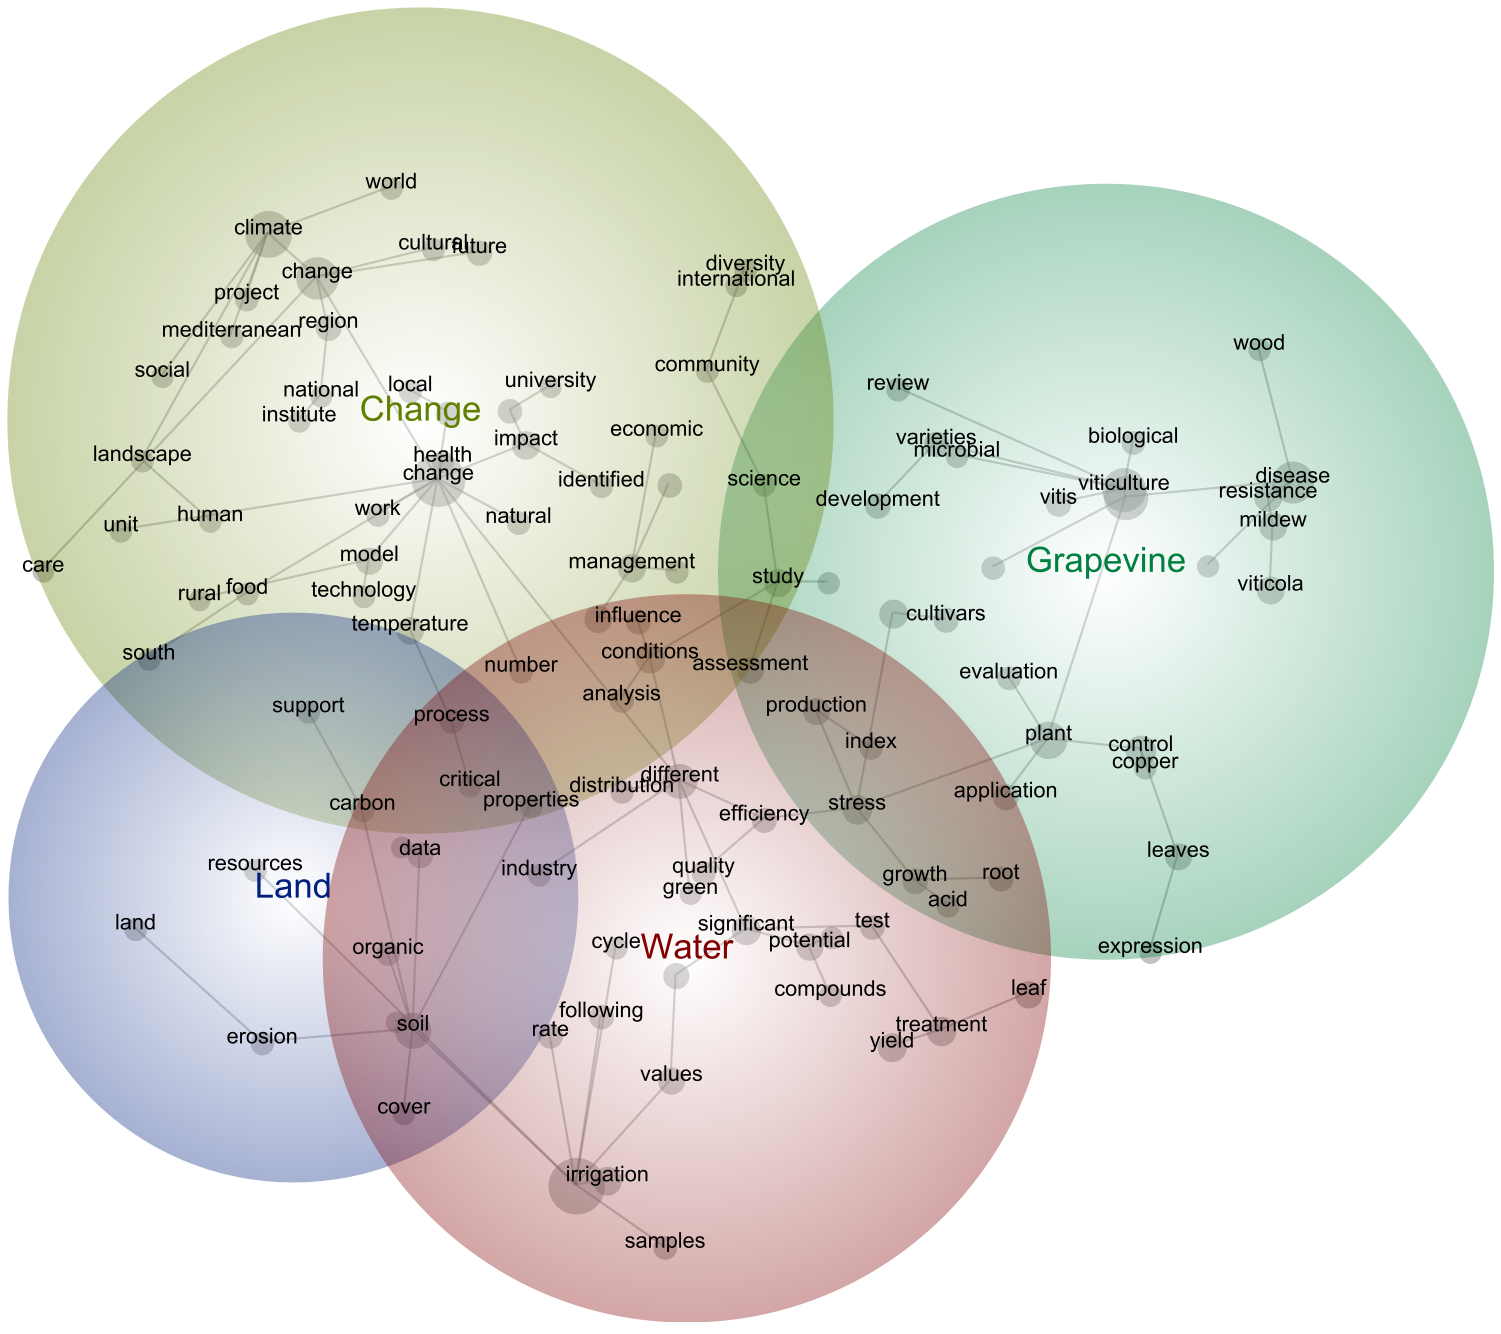
\includegraphics[width=\linewidth]{Winegrowing-concept-map}
    \caption{Your caption here}
    \label{fig:lexi}
\end{figure}

        TODO: write a summary description of the leximancer outputs.

\subsection{Key Factors Impacting Environmental Sustainability in Australian Winegrowing}
    % What are the primary factors that significantly impact environmental sustainability in the Australian winegrowing industry?
    %     Purpose: Identify the most influential variables directly affecting environmental sustainability and those that are perceived to directly impact environmental sustainability.
    %     Results: Review the most influential factors and what they are related too. Compare this to the data in SWA.

    % What are the relationships between these factors in the Australian winegrowing industry?
    %     Purpose: Explore and understand the causal and correlated relationships among the factors.
    %     Results: Use the generic BN to illustrate the overall agreed upon relationships between discussed factors.

\begin{figure}[h!]
    \centering
    % \includegraphics[width=\textwidth]{path_to_coonawarra_bn_figure} % Adjust the width as needed
    \caption{The resultant Bayesian network after initial discussions of how factors that contribute to environmental impact are related. Illustrating the general relationships that exist between vineyard factors and environmental impact in Australian winegrowing.}
    \label{fig:generalBN}
\end{figure}


The relationships between the nodes defined by the industry panel are depicted in~\ref{figure:generalBN}. The figure highlights which factors are influenced by others. For instance the key factors influencing environmental impact centre around the application of agrochemical sprays, soil management, pest/disease and water. It also illustrates the complex nature of variables such as water and their interrelatedness.

The BN provided a comprehensive overview of how these factors interact, showing not only direct relationships but also how changes in one factor can propagate through the network to affect others. This understanding is crucial for developing targeted interventions and policies aimed at improving sustainability in the winegrowing industry.

By using the generic BN, the study was able to illustrate the complexity of interactions that define environmental sustainability in Australian winegrowing.

% Comparing this with the data from Sustainable Winegrowing Australia (SWA), it was evident that the factors identified in the BN align with the critical areas SWA focuses on, such as water use, greenhouse gas emissions, and agrochemical use. This alignment reinforces the importance of these factors and supports the findings of the BN analysis.
% What are the relationships between these factors in the Australian winegrowing industry?

% Purpose: Explore and understand the causal and correlated relationships among the factors.

The bibliometric analysis using Leximancer, revealed key concepts and their relevance to environmental sustainability in the Australian winegrowing industry. The most prominent concept was water. The critical importance of other variables being measured by their comparative appearance in articles relative to water (making water 100\%).

Other significant concepts included "change", "climate", and "disease". These terms highlight the focus on adapting to climate change and managing plant diseases, both of which are crucial for maintaining sustainable practices (see \ref{tab:lexi}). Furthermore, change and climate were kept separate to illustrate the variety of different chagings such as in practice, legislation and resource abundance. Additionally, although not in the top 10; "soil", "region", "practices", and "legislation" also appear to be dominant features within the literature. These factors are critical as they shape the environmental strategies employed by vineyards.

The major concepts of these features was change, grapevine, water and land (see Figure \ref{fig:lexi}). these concepts illustrate the overarching theme between how the different concepts are connected, which showed very similar themes to that of the industry panel. A key difference was the rarity in how secondary and tertairy drivers of industry such as fuel or electricity use, were connected to primary sustainable concerns such as disease. With these conceps being related to the operations in fields as a result of changing practices or implementing different pest controls.

Together these outputs provide a comprehensive overview of the key factors affecting environmental sustainability in the Australian winegrowing industry, offering valuable insights into areas of focus and potential improvement. This analysis underscores the multifaceted nature of sustainability, highlighting both the primary concerns and the interconnected secondary factors that must be managed on the ground.

\subsection{Sustainability specifics: Coonawarra Winegrowing}

Located in South Australia's Limestone Coast zone, Coonawarra is characterised by its cooler Australian climate and the unique geology of the limestone coast, which provides an excellent foundation for viticulture. The Coonawarra winegrowing region is renowned for its exceptional wine quality, particularly its Cabernet Sauvignon \cite{hallidayAustralianWineEncyclopedia2009}. Due to the region's distinct characteristics and the expert panels' expertise, this region was the ideal case study for applying Bayesian Networks using the expert panels overarching ideas around environmental sustainability practices to specific regional factors.

In this case study, we apply BN to model and analyze the complex interactions between various environmental factors affecting wine production in Coonawarra. By incorporating industry-specific data and expert knowledge, the BN framework allows us to quantify the impacts of key variables such as water use, agrochemical application, soil health, and climate conditions to each other. This approach not only aids in understanding the current sustainability status of the region but also helps in identifying potential areas for improvement and implementing effective management strategies.

The insights gained from this case study can serve as a valuable reference for other winegrowing regions aiming to enhance their environmental sustainability practices through the use of advanced probabilistic models like Bayesian Networks.

    %     Sustainability in Coonawarra Winegrowing: Key Factors and Influences
    % #TODO: what are the regional specifics of coonawarra
    % How do the identified key factors vary across different wine regions in Australia, and what regional characteristics influence these variations?
    %     Purpose: Examine regional differences and tailor sustainability strategies.
    %     Results: Compare the generic model to the Coonawarra model. Acknowledge there is more work to be done here due to the amount of regions across Australia and the world. Prevous work also helps to illustrate these differences.

    % How do changes in key factors under various environmental and regulatory scenarios influence the overall environmental impact in Coonawarra?
    %     Purpose: Assess different factors overall influence to environmental sustainability given the definitions used.
    %     Results: Use the CPT values to assess the significant contribution of different variables on the BN and how that effects environmental sustainability.

\begin{figure}[h!]
    \centering
    % \includegraphics[width=\textwidth]{path_to_coonawarra_bn_figure} % Adjust the width as needed
    \caption{Coonawarra-specific Bayesian Network illustrating key factors impacting environmental sustainability, with nodes coloured by sensitivity to environmental impact.}
    \label{fig:coonawarra_bn}
  \end{figure}

% TODO: the exclusion of renewable fuels due to none being used in coonawarra
% the difference in vineyard floor management and its relationship to tractors
% The influence of compost, soil depth and clay content. although not specifically significant due to not listing the CPTs - it was highlighted as significant with different influence values depending on the direct field in question and not just which vineyard.
% variation occurs all the way to the vine level!

  This subsection examines how the identified key factors impacting environmental sustainability vary across different wine regions in Australia, with a focus on Coonawarra. By comparing the generic Bayesian Network (BN) model to the Coonawarra-specific model (Figure \ref{fig
  } and Figure \ref{fig
  }), we identify regional characteristics that influence these variations.
  
The comparison reveals that while some factors, such as water use and agrochemical legislation, remain consistently significant, other factors such as soil show variation not only at a regional level but sometimes at the paddock level as described by the expert panel. The Coonawarra model highlights the unique environmental and regulatory conditions specific to this region, indicating a need for tailored sustainability strategies. It is important to acknowledge that this analysis also illustrates that further work would be required to describe other regions or specific vineyards. 

The CPT values allow for an in-depth analysis of how changes in key factors, under various environmental and regulatory scenarios, influence the overall environmental impact. For instance, the Coonawarra-specific model demonstrates that the significance that pest/disease, and agrochemicals have a higher sensitivity to environmental impact compared factors such as green house gas emissions. Importantly that these sensitive factors also link greatly to one another, highlighting how critical areas for regulatory and environmental interventions can be to multiple factors beyond their specific target.
  
By using Conditional Probability Tables (CPTs) within the BN, the significant contributions of different variables to environmental sustainability in Coonawarra were assessed. Figures \ref{fig
  } and \ref{fig
  } illustrate these networks with nodes coloured according to their sensitivity values relative to environmental impact.

In the Coonawarra-specific BN, the most significant factors impacting environmental sustainability are water quality, pest and disease management, market pressures, agrochemical use, and climate/weather conditions. These factors were identified as having the highest sensitivity to environmental impact, indicating their crucial roles in the sustainability of the region.

The primary difference in interactions between the two BNs (see Figure~\ref{fig:robyn} and~\ref{fig:marcel}) lies in vineyard floor management and tractor passes. In one, more tractor passes were used purposefully to manage the vineyard floor; the other managed vineyard floor as a consequence of tractor passes, leveraging opportunities when the tractor was used. This distinction highlights how operational decisions can vary based on regional practices and priorities. A point was also raised that scale can cause a further driving factor, where tractor passes may be greatly increased as an expense on larger plots of land. However, this issue as well as directly attributing measurable cause to granular specifics such as composting, soil depth and clay content cannot be fully addressed without site or paddock specific knowledge.

As a factor, water emerged as the most interconnected variable for both BNs, with edges connecting it to almost everything either directly or indirectly, illustrating its fundamental role in agriculture. The edges between different factors reveals that water is the most connected. Weather conditions also play a significant role, influencing water availability, quality and disease/pest pressures.

The Coonawarra-specific BN supports the findings from the literature, with a more structured map of how factors interact compared to the automatically generated figures from tools like Leximancer. The BN provides a detailed view of the relationships between factors, highlighting the central role of water and the interconnectedness of pest management, market pressures, and climate conditions. Additionally, the BNs emphasise economic factors, such as market pressures and grape prices, and includes how they interact within a scope of secondary factors like fuel and electricity use.

% The other case study BN aligns with the literature by visually representing connections and highlighting significant factors through bibliometric analysis. However, the BN derived from the industry panel offers explicit connections and sensitivity analyses based on expert knowledge, providing a more nuanced understanding of the factors and their impacts compared to the broader mind maps generated from literature reviews.

The two case study BNs are almost identical in their significant factors and interactions. Both emphasize the importance of water quality, pest and disease management, and climate conditions. The primary difference is the sensitivity to tractor passes, water quality, water scarcity, and soil degradation management, with one model showing higher sensitivity to these factors. Aside from the role of tractor passes, there are no major differences between the two BNs. The similarity in significant factors and their interactions underscores the robustness of the BN approach in capturing the critical elements of environmental sustainability in winegrowing.

The findings from the case study align closely with the literature, illustrating more directly how factors that contribute to environmental sustaianbility are connected. The BNs provide a detailed and structured view of primary factors and their relationships to secondary and tertiary concerns within the industry. This detailed evaluation helps prioritise actions and policies that could lead to significant improvements in the sustainability practices of winegrowing regions.

% =================================
Structuring the Results Section Based on These Questions:
Introduction to Results

    Content: Briefly restate the refined research questions.
    Explanation: Explain the approach to answering these questions using the BN model and CPT values.

Primary Factors Identification

Question: What are the primary factors that significantly impact environmental sustainability in the Australian winegrowing industry?

    Content: Present the primary factors identified through your analysis.
    Data: Use the rigorous definitions and the generic BN to highlight these factors.
    Figures/Tables: Include a table or figure showing the key factors and their relative importance.

Quantitative Measurement and Analysis

Question: How can these key factors be quantitatively measured and analyzed to assess their contributions to sustainability in the Australian winegrowing industry?

    Content: Describe the methods used to measure and analyze the key factors.
    Data: Show measurements and analytical results from the CPT values in the specific BN models.
    Figures/Tables: Include charts or tables showing the measurements and analyses.

Relationships Between Factors

Question: What are the direct and indirect relationships between these key factors and environmental sustainability in the Australian winegrowing industry?

    Content: Discuss the direct and indirect relationships identified.
    Data: Present interaction diagrams or tables.
    Figures/Tables: Include a BN tree diagram illustrating these relationships.

Regional Variations

Question: How do the identified key factors vary across different wine regions in Australia, and what regional characteristics influence these variations?

    Content: Compare the key factors and their impacts across different regions.
    Data: Present comparisons between the two specific BN models from different growers.
    Figures/Tables: Include figures comparing regional differences.

Scenario Analysis

Question: How do changes in key factors under various environmental and regulatory scenarios influence the overall environmental impact in the Australian winegrowing industry?

    Content: Analyze the impact of different scenarios on environmental sustainability.
    Data: Use scenario-based BN queries to show changes in key factors and their impacts.
    Figures/Tables: Include charts or tables summarizing the scenario analysis results.

Example Framework for Presenting Results:
Introduction to Results

"The results of this study are structured to address five primary research questions aimed at understanding the key factors and their interactions affecting the environmental impact of vineyards in the Australian winegrowing industry. The analysis leverages Bayesian Network models to provide a comprehensive view of these factors and their contributions."
Primary Factors Identification

Question: What are the primary factors that significantly impact environmental sustainability in the Australian winegrowing industry?
Results:

    Identified Factors: Water usage, pesticide application, soil management, etc.
    Data Source: Defined terms provided by industry experts and the generic BN model.
    Figures: Table 1 shows the key factors and their relative importance derived from the BN analysis.

Quantitative Measurement and Analysis

Question: How can these key factors be quantitatively measured and analyzed to assess their contributions to sustainability in the Australian winegrowing industry?
Results:

    Measurements: Quantitative analysis of key factors using CPT values from two specific BN models.
    Data Source: CPT values from BN models of two growers.
    Figures: Table 2 presents the measurements and analysis results.

Relationships Between Factors

Question: What are the direct and indirect relationships between these key factors and environmental sustainability in the Australian winegrowing industry?
Results:

    Interactions: Direct and indirect relationships as illustrated by the BN model.
    Data Source: Generic BN model and specific models.
    Figures: Figure 1 illustrates the BN tree diagram showing these relationships.

Regional Variations

Question: How do the identified key factors vary across different wine regions in Australia, and what regional characteristics influence these variations?
Results:

    Regional Variability: Comparison of factors and impacts across regions using specific BN models.
    Data Source: BN models from two growers in different regions.
    Figures: Figure 2 compares the BN models for different regions.

Scenario Analysis

Question: How do changes in key factors under various environmental and regulatory scenarios influence the overall environmental impact in the Australian winegrowing industry?
Results:

    Scenarios: Impact analysis under different scenarios using BN models.
    Data Source: Scenario-based BN queries.
    Figures: Table 3 summarizes the scenario analysis results.

This refined approach ensures that your Results section directly addresses your research questions and clearly presents your findings. Let me know if there are specific details or sections you’d like further refined!

\section{Title}
A Bayesian Network Model based decision support tool for Environmental Sustainability in the Australian Winegrowing Industry.

\section{Abstract}

The assessment of environmental sustainability in the Australian winegrowing industry remains a complex issue involving changing and compounding factors. To address this, we developed a Bayesian Network (BN) using data and expert elicitation to summarise the key factors, their relationships, and how they come together to influence vineyards' environmental outcomes. The study leveraged diverse expert perspectives to mitigate biases in probability estimations and promote discourse.

The development of the BN involved an iterative process, including variable selection and definition, the defining of model structure and variable relationships, and finally the determining of relationship significance through probabilities. Expert input was pivotal in structuring the BN model, ensuring relevance to industry, and how a variables influence changed across regions and scenarios.

Due to the possible variation in any given vineyard scenario the BN model was expanded to review a case study of the Coonawarra wine region in South Australia. This highlighted regional differences between growers whilst also maintaining the significance of industry-wide concerns such as the use of agrochemicals. To promote accessibility and scrutiny the BN was further developed into an application, allowing the possibility of further industry and stakeholder feedback; enabling a systematic re-evaluation of significant factors to the wine growing industry and how they change over time.

